%% Creator: Inkscape inkscape 0.48.3.1, www.inkscape.org
%% PDF/EPS/PS + LaTeX output extension by Johan Engelen, 2010
%% Accompanies image file 'gputile.pdf' (pdf, eps, ps)
%%
%% To include the image in your LaTeX document, write
%%   \input{<filename>.pdf_tex}
%%  instead of
%%   \includegraphics{<filename>.pdf}
%% To scale the image, write
%%   \def\svgwidth{<desired width>}
%%   \input{<filename>.pdf_tex}
%%  instead of
%%   \includegraphics[width=<desired width>]{<filename>.pdf}
%%
%% Images with a different path to the parent latex file can
%% be accessed with the `import' package (which may need to be
%% installed) using
%%   \usepackage{import}
%% in the preamble, and then including the image with
%%   \import{<path to file>}{<filename>.pdf_tex}
%% Alternatively, one can specify
%%   \graphicspath{{<path to file>/}}
%% 
%% For more information, please see info/svg-inkscape on CTAN:
%%   http://tug.ctan.org/tex-archive/info/svg-inkscape
%%
\begingroup%
  \makeatletter%
  \providecommand\color[2][]{%
    \errmessage{(Inkscape) Color is used for the text in Inkscape, but the package 'color.sty' is not loaded}%
    \renewcommand\color[2][]{}%
  }%
  \providecommand\transparent[1]{%
    \errmessage{(Inkscape) Transparency is used (non-zero) for the text in Inkscape, but the package 'transparent.sty' is not loaded}%
    \renewcommand\transparent[1]{}%
  }%
  \providecommand\rotatebox[2]{#2}%
  \ifx\svgwidth\undefined%
    \setlength{\unitlength}{222.14212036bp}%
    \ifx\svgscale\undefined%
      \relax%
    \else%
      \setlength{\unitlength}{\unitlength * \real{\svgscale}}%
    \fi%
  \else%
    \setlength{\unitlength}{\svgwidth}%
  \fi%
  \global\let\svgwidth\undefined%
  \global\let\svgscale\undefined%
  \makeatother%
  \begin{picture}(1,0.91280988)%
    \put(0,0){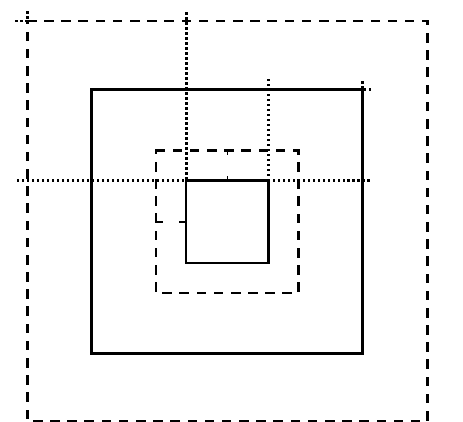
\includegraphics[width=\unitlength]{figs/gputile.pdf}}%
    \put(0.47542287,0.48195855){\color[rgb]{0,0,0}\makebox(0,0)[lb]{\smash{$w^\prime$}}}%
    \put(0.41017324,0.41856853){\color[rgb]{0,0,0}\makebox(0,0)[lb]{\smash{$h^\prime$}}}%
    \put(0.4803591,0.54175468){\color[rgb]{0,0,0}\makebox(0,0)[lb]{\smash{$r$}}}%
    \put(0.35895388,0.41856853){\color[rgb]{0,0,0}\makebox(0,0)[lb]{\smash{$r$}}}%
    \put(0.66952792,0.73183289){\color[rgb]{0,0,0}\makebox(0,0)[lb]{\smash{$rt^\prime$}}}%
    \put(0.79867196,0.61451188){\color[rgb]{0,0,0}\makebox(0,0)[lb]{\smash{$rt^\prime$}}}%
    \put(0.20258068,0.88151657){\color[rgb]{0,0,0}\makebox(0,0)[lb]{\smash{$iw^\prime$}}}%
    \put(-0.00185692,0.68488735){\color[rgb]{0,0,0}\makebox(0,0)[lb]{\smash{$jh^\prime$}}}%
    \put(0.46888112,0.34857001){\color[rgb]{0,0,0}\makebox(0,0)[lb]{\smash{tile}}}%
    \put(0.41001713,0.29263789){\color[rgb]{0,0,0}\makebox(0,0)[lb]{\smash{halo region}}}%
    \put(0.40174748,0.16167496){\color[rgb]{0,0,0}\makebox(0,0)[lb]{\smash{enlarged tile}}}%
    \put(0.42717077,0.02343624){\color[rgb]{0,0,0}\makebox(0,0)[lb]{\smash{2D array}}}%
  \end{picture}%
\endgroup%
